% .:: Laden der LaTeX4EI Formelsammlungsvorlage
\documentclass[fs, footer]{latex4ei}

% Dokumentbeginn
% ======================================================================
\begin{document}


% Aufteilung in Spalten
\begin{multicols}{4}
	\fstitle{Nanoelectronics}
	
\vspace{-2mm} % Man muss optimieren wos nur geht ;)
% -------------------------------------------
% | 	Nanoelectronics					|
% ~~~~~~~~~~~~~~~~~~~~~~~~~~~~~~~~~~~~~~~~~~~
%=======================================================================

\emphbox{
	\textbf{HINWEIS:} Die Formelsammlung ist eine einfache Mitschrift, sehr ungeordnet und kann grobe Fehler enthalten. Sie dient lediglich als Überblick zum Fach.
	Wenn jemand die FS ergänzen/überarbeiten möchte, einfach melden
}


Wichtige Begriffe: 
\begin{tabular}{ll}
	dispersion & Verteilung\\
	lattice & Kristallgitter\\
	impurities & Fremdstoffe\\
	to scatter & streuen\\
\end{tabular}

Abkürzungen:
\begin{tabular}{ll}
	CVD & chemical vapour deposition\\
	CNT & carbon nanotube\\
	DoS & Density of States\\
	HOPG & Highly Ordered Pyrolytic Graphite\\
	PMMA & Polymethylmethacrylat (Acrylglas)\\
	STM & Scanning tunneling microscope\\
\end{tabular}


\section{Moores Law -- scaling}

1. Transistormaterial: Germanium\\
Transistor scaling 22nm between drain and source of a MOSFET\\
scaling cant continue indefinitely
Against Moores Law: the rising costs of fabrication, the limits of lithography, and the size of the transistor.
Advantages of scaling: smaller, cheaper, and faster and to consume less power.








\section{Quantum mechanics}
	Klassische Bewegungsgleichung: $m \frac{\diff^2 \vec r(t)}{\diff t^2} = \vec F$\\
	Classical wave equation:\\
	\boxed{ \frac{1}{c^2}\frac{\partial^2\Psi}{\partial t^2} - \sum\limits_{i=1}^n \frac{\partial^2\Psi}{\partial x_i^2} = 0 }
	\boxed{ \begin{array}{l} c = \lambda f \\ \omega = 2\pi f \end{array}} \boxed{k = \frac{2\pi}{\lambda}}
	Waves behave as particles. Electrons and photons are both, particles and waves.\\
	Electron Orbits: $mvr = n \hbar$ \quad $n \lambda = 2 \pi r$\\
	Bohr atom model: \boxed{ E_n \approx -13.6 \frac{Z^2}{n^2} \si{\electronvolt} } \qquad $Z$: count of protons\\
	De Broglie Wavelength: $h = p \lambda$ \quad $p = \hbar k$ \quad $h = 2\pi \hbar$\\
	Uncertainty principle: \boxed{ \Delta x \cdot \Delta p_x \ge \frac{\hbar}{2} } \qquad $\Delta E \cdot \Delta t \ge \frac{ \hbar }{2}$\\
	transistor dimension: $L_{crit} \approx \frac{h}{\sqrt{2m^* E_b}} \approx \SI{4}{\nano \meter}$\\ with $m^* \approx 0.19m_0$ \quad $E_b = 0.5eV$\\ 

	\subsection{Schroedinger Equation}
	\begin{equation}
		\left( \frac{-\hbar^2}{2m} \nabla^2 + V(\vec r,t)  \right) \Psi(\vec r,t) = \i \hbar \frac{\partial}{\partial t} \Psi(\vec r,t)
	\end{equation}
	Potential energy $V(\vec r,t) \in \R$ \qquad (for Hydrogenatom $V(\vec r) = \frac{-e^2}{r}$)\\
	Hamiltonian $\hat H = \left( \frac{-\hbar^2}{2m} \nabla^2 + V(\vec r,t)  \right)$\\
	Probabilitydensity $P(\vec r,t) = \Psi(\vec r,t) \cdot \Psi^* (\vec r,t) = |\Psi^2|$\\
	Normalized: $\int |\Psi(\vec r)|^2 \diff \vec r = 1$\\
	
		\subsubsection{time-independent Schroedinger equation}
		if $V(\vec r,t)$ is time-independent:\\
		$\Psi(\vec r,t) = \Psi(\vec r) \exp\left(\frac{\i E t}{\hbar}\right)$ \quad $\Ra$ \quad $\hat H \Psi(\vec r) = E \Psi(\vec r)$\\
		\\
		1D Confinement (infinite Quantum Well):\\
		$\Psi_n(x) = \sqrt{\frac{2}{L_x}} \sin \left( \frac{\sqrt{2mE}}{\hbar} x \right)$\\
		$E_n = \frac{\hbar}{2m} k_n^2 = \frac{\hbar^2 \pi^2 n^2}{2mL}$\\
		\\
		2D Confinement
		$\Psi(x,y) = \sqrt{\frac{4}{L_x L_y}} \sin(k_x x) \cdot \sin(k_y y)$\\
		$E_n = \frac{\hbar}{2m} (k_x^2 k_y^2)$\\
		\\
		$\delta$-D Confinement wirh $\eset{i=x,y,...,\delta}$\\
		$\Psi(\vec r) = \sqrt{\frac{2\delta}{ \prod L_i }} \prod\limits_{i=1}^\delta \sin(k_i \cdot i)$\\
		$E_n = \frac{\hbar}{2m} (k_x^2 k_y^2)$\\
		
		Analytical solutions are only possible for the infinite quantum well

	\subsection{Quantenphysik}
	$E_{Ph}=f\cdot h= \hbar \cdot \omega = \frac{hc}{\lambda}$ \qquad \boxed{ \lambda \cdot \vec p = h }\\
	$p = \hbar k = \frac{hk}{\lambda}$ \qquad $\hbar = \frac{h}{2\pi}$ \qquad $k=\frac{2\pi}{\lambda}$\\



	\subsection{Phonons}
	are quasiparticles to describe modes of vibrations of elastic structures of interacting particles.
	there are acoustic and optical phonons.



	\section{Semiconductors}
	
		\subsection{bandstructure}
	Fermienergie $F_E$: Höchste Energie eines Elektrons bei $T = 0K$
	Isolator: große Bandlücke $E_G > 3$eV
	Halbleiter: kleine Bandlücke $1 eV < E_G < 3eV$ kann durch thermische Energie überwunden werden		
	
	
	
	Materials in columns: \\ IV: Si,Ge, III-V(GaAs, InP, GaN(BluRay), InSB),II-VI(CdSe, CsTe) IV-VI(PbS,PbSe)\\
	Silicon in crystal structure: 5 per Cube\\
	Chemical band structure: energylevels of diffrent atoms moving close together\\
	At finite temperature some electrons can move around. $n \propto \exp(T b_{gap})$\\
	At $300K:n = 1.5 \times 10^10 cm^3$\\
	doping with donors(P,As) or acceptors(B,In) to lower the energy for emission or capture an electron\\
	atoms: $10^23$ per cm$^3$, dopants: $10^15$ per cm$^3$\\
	\\
	$E_{kin} = \frac{p^2}{2m} = \frac{\hbar^2 k^2}{2m}$ \qquad  $\frac{\diff^2 E}{\diff p^2} = \frac{1}{m}$\\
	Effektiv mass: $\frac{1}{m^*_{eff}} = \frac{1}{\hbar} \cdot \frac{\diff^2 E}{\diff k^2}$\\
	
	
	Resistorequation: $R_{Mat} = \rho_{Mat} \frac{l}{wt}$\\
	conductivity: $\sigma = \frac{1}{\rho} = q \mu_n n_i$\\
	resistivity: $\rho$\\
	
	uncrtainity for electron: $\Delta x \ge \frac{0.5 \cdot 10^{-4}}{\Delta v}$\\
	
	
	$v_{sat}$ for Si: $2 \cdot 10^7 \frac{cm}{s}$\\
	$I_{DS} = \frac{1}{2} \mu C_{ox} \frac{W}{L} (V_{DD} - V_T)^2$\\
	$P = V^2_{DD} C_{ox} f_{max}$\\
	
	
\section{Transistors}
$I_D = \frac{1}{2} \mu_n C^{'}_{ox} \frac{W}{L} \cdot (V_{GS} - V_{th})^2$\\
$\mu_n \approx 250 \cdot 10^{-4} \frac{m^2}{Vs}$, $\mu_p \approx 100 \cdot 10^{-4} \frac{m^2}{Vs}$\\
$P_{cap} = \alpha_{01} f C_{ox} V_{DD}^2$\\
$f_{max} = \frac{I_{sat}}{V_{DD} C_{ox}}$

	
	\subsection{scaling with factor $S < 1$}
	
	reduce area $A = W \cdot L$ \quad $A' = A \cdot S^2$\\
	increase speed $\tau = \frac{L}{v}$ \quad $\tau' = \tau \cdot S$\\
	reduce power $P = VI\tau$ \quad $P' = P \cdot S^3$\\
	
	
	Transistorscaling in nm: 90(2003), 65(2005), 45(2007), 32(2009), 22(2011) 
	
		
		\subsubsection{Problem of scaling}
		\begin{enumerate}
			\item Tunneling across the oxide
			\item Need for new lithographic techniques
			\item Parasitic effects due to inteconnects
			\item Melting interconnects due to voids
			\item High field and breakdown effects
		\end{enumerate}
		$\Ra$ new materials, processes and technologies needed!

		High-K Material (high dielectric $\varepsilon$) as Gate isolator:
		$\Ra$ $1,6 \cdot C_G$, $0.01 \cdot I_{leak}$\\
		
		%siehe slide 4, seite 12 und sl4, p19
		Example Intels 45nm MOSFET:
		High-K with silicon gaten:
		Problems: uneven 


	Form: Normalgate, Dualgate, Trigate\\
	Best: Surrounding Gate: CNT -- high-K -- metal-gate\\

	
	\subsection{Silicon Nanowire}
		Fabrication: growth on a gold(Au) particle
	
	
	\subsection{GaN - Transistors}
	Why GaN?
	\begin{itemize}
		\item Wide bandgaps of GaN and AlGaN (high breakdown volt.)	
		\item high drift velocity(hf)
		\item strong piezoelectric effekt
		\item High temperature operation
	\end{itemize}

	HEMT-Transistor: Two substrate materials, doped and undoped\\
	$\Ra$ electrons move on a 2D-Sheet\\
	Cut-Off-Frquency $f_T = \frac{v_{sat}}{2\pi L_g}$: $g_m = 1$ (no amplification anymore)\\
	Oxide-Capacitance $C_{ox} = \frac{\varepsilon_0 \varepsilon_r}{t_{ox}}$\\
	T-Gate: smooth electric field in the channel. 
	
	


	
	
	\subsection{Quantum Wire}
	Ideal: just one subband in two dimensions
	But for good conductance(mobility, drift velocity) one need $~20nm$
	Fabrication Methods: Stressor, Etching, Ion implantation, Vicinal Growth
	
	
	Split Gate Transistor: 1D tunnel in the gate between source and drain.
	electron wave transistor: 
	
	
\section{Graphene}
2D Network of 3D Carbon Atoms.\\
Stacked Layers of Graphene form Graphite.\\
applications: seperation membranes, capacitors
	
	\hspace{-0.2cm}\pbox{4.0cm}{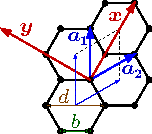
\includegraphics{./img/graphene.pdf}} \quad 
	\pbox{5.0cm}{ $b \approx \SI{0.14}{\nano \meter}$ \\[0.5em] $d = 2b \approx \SI{2.8}{\nano \meter}$ \\[0.5em] 
	$\vec a_1 = \frac{3}{2} b \vec x + \frac{\sqrt{3}}{2}b \vec y = \frac{\sqrt{3}}{2}a \vec x + \frac{1}{2}a \vec y$ \\[0.5em]
	$\vec a_2 = \frac{3}{2} b \vec x - \frac{\sqrt{3}}{2}b \vec y = \frac{\sqrt{3}}{2}a \vec x - \frac{1}{2}a \vec y$ \\[0.5em]
	$\norm{\vec a_1} = \norm{\vec a_2} = a = \sqrt{3}b \approx \SI{0.246}{\nano \meter}$ \\[0.5em] $\norm{\vec x} = \norm{\vec y} = 3b$ }
	
		\subsection{Properties}
		thinnest material sheet imagineable\\
		extremly strong (5 times stronger than steel)\\
		semimetall: better conduction than metal, can switched ON and OFF\\
		very light, good head conductor
		size of one cell: edge $d \approx 0.14nm$, edge2edge $a = \sqrt 3 d$\\
		
		
		\subsection{production}
		\begin{itemize}
			\item Exfoliated Graphene: peeling HOPG with foil. Good for scienece not for manufacturing
			\item Epitaxial growth: silicon carbide($\mathrm{SiC}$) is heated ($>1100 {}^\circ$C) to reduce it to graphene.
		\end{itemize}
	
	\subsection{Carbon-Nano-Tubes CNT}
	Propertys: diameter: $d \approx \SI{10}{\nano \meter}$\\
	Application: wires, transitors, sensors, Molecular tweezers
	Single Walled and Multiwalled:
	SWCNT: single layer of graphite(graphene) rolled up as cylinder\\
	\\
	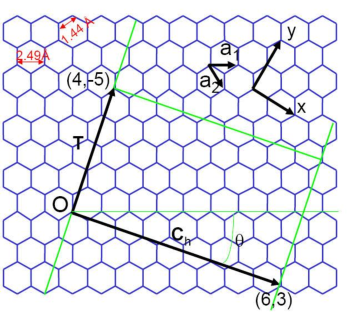
\includegraphics{./img/chirality.pdf}
	\\
	Kind of curls: zig-zag $(n,0)$, armchair $(n,n)$, quiral $(n,m)$\\
	chiral vector (tube circumfence): $\vec C_h = n \vec a_1 + m \vec a_2$\\
	translation vector $\vec T = [(2m+n) \vec a_1 -(2n+m) \vec a_2] / \gcd(n,m)$\\
	Tube-Diameter: $d_T = \frac{\norm{\vec c_h}}{\pi} = \frac{a}{\pi} \sqrt{n^2 + nm + m^2}$ \quad with $a = 0.246$nm\\
		
	Kind of Nanotube: $\begin{cases} \text{metalic} & \text{if}\ (n-m)/3 \in \N_0 \\ \text{semiconductor} & \text{else} \end{cases}$\\
	Bandenergy in dependency of $\vec k$: \\
	$E(\vec k) = \varepsilon_0 \pm t \sqrt{1+4\cos\left( \frac{\sqrt{3} a k_x}{2} \right)  \cos\left( \frac{ a k_y}{2} \right) + 4\cos^2\left( \frac{a k_y}{2} \right) }$\\
	Periodic Boundary Conditions: $\vec C^\top_h \bdot \vec k = 2 \pi n$\\
	
	% tobias.haerbele@nano.tum.de

% Ende der Spalten
\end{multicols}

% Dokumentende
% ======================================================================
\end{document}
